% !TEX root = ../eval.tex

\section{Methods}%
\label{sec:data}

\subsection{Data}%
\label{sub:data}

\paragraph{Dataset description:}%
\label{par:dataset_description}

I use data from a UK-based financial management app that allows users to link
accounts from different banks to obtain an integrated view of their finances.
The complete dataset contains more than 500 million transactions made between
2012 and June 2020 by about 250,000 users, and provides information such as
date, amount, and description about the transaction as well as account and
user-level information. Crucially for this paper, the app can access up to
three years of historic data for each linked account.

The main advantage of the data for the study of consumer financial behaviour is
that we can observe user behaviour at the transaction level across all their
accounts, and that the data is automatically collected rather than collected
through a survey.

The main limitation is the non-representativeness of the sample relative to the
population as a whole. Financial management apps are known to be used
disproportionally by men, younger people, and people of higher socioeconomic
status \citep{carlin2019generational}. Also, as pointed out in
\citet{gelman2014harnessing}, a willingness to share financial information with
a third party might not only select on demographic characteristics, but also
for an increased need for financial management or a higher degree of financial
sophistication. Because our analysis does not rely on representativeness, we do
not address this.\footnote{For an example of how re-weighing can be used to
mitigate the non-representative issue, see \citet{bourquin2020effects}.}


\paragraph{Cleaning:}%
\label{par:cleaning}

I use the dataset described above for a number of projects, and perform a
number of steps to create a minimally cleaned version of the dataset that is
the basis for all such projects. These steps are performed in a dedicated
data repository and not run as part of this project, but the module with
all cleaning functions is available in the project directory.\footnote{Link to
    cleaning functions:
\href{https:/egithub.com/fabiangunzinger/mdb_eval/blob/f51e49c95c5884d2dc417be23921a8acd85aec9d/src/data/clean.py}{\faGithub}}

Here, I briefly describe the main cleaning steps and their rationale. I drop
all transactions with a missing description string because these cannot be
categoriesed, and all transactions that are not automatically categoriesed by
the app. Dropping these transactions makes is likely that we will underestimate
amounts spent and saved, but minimises the risk of incorrectly classified
transactions. I group transactions into transaction, spend, and income
subgroups. Spend subgroups are defined following \citet{muggleton2020evidence};
income subgroups, following \citet{hacioglu2020distributional}.\footnote{Link
to classification file:
\href{https://github.com/fabiangunzinger/mdb_eval/blob/92af366d4c4052cc7a7f78a6178086de8ecdfb75/src/data/txn_classifications.py}{\faGithub}}
Finally, I classify as duplicates and drop transactions with identical user ID,
account ID, date, amount, and transaction description. This will drop some
genuine transactions, such as a user buying two identical cups of coffees at
the same coffee shop on the same day. However, data inspection suggests that in
most cases, we remove genuine duplicates.


\paragraph{Sample selection:}%
\label{par:sample_selection}

We select our sample so as to include users for whom we can be reasonably
certain that we observe all relevant financial transactions, and do so for at
least six months before and after they sign up to the app. In addition to that,
we exclude users who might use the app for business purposes as well as
pensioneers, whose financial objectives might be different.

\begin{table}
\centering
\caption{Sample selection}\label{tab:selection}
\begin{tabular}{lrrrr}
\toprule
                                       &  Users & User-months &       Txns & Txns (m\pounds) \\
\midrule
                            Raw sample & 27,175 &     795,338 & 65,972,558 &          12,527 \\
             Drop first and last month & 26,565 &     741,170 & 64,157,932 &          12,179 \\
  At least 6 months of pre-signup data & 11,835 &     310,517 & 29,244,871 &           5,743 \\
 At least 6 months of post-signup data &  6,404 &     195,050 & 19,681,242 &           3,957 \\
          At least one current account &  5,833 &     178,845 & 18,257,300 &           3,738 \\
          At least one savings account &  4,506 &     138,181 & 14,485,916 &           3,133 \\
At least \pounds5,000 of annual income &  1,877 &      57,064 &  6,493,155 &           1,386 \\
           At least 10 txns each month &  1,686 &      51,190 &  5,935,336 &           1,262 \\
  At least \pounds200 of monthly spend &  1,478 &      44,641 &  5,333,532 &           1,135 \\
      Complete demographic information &  1,240 &      38,087 &  4,598,590 &             952 \\
                           Working age &  1,219 &      37,377 &  4,529,599 &             929 \\
                          Final sample &  1,219 &      37,377 &  4,529,599 &             929 \\
\bottomrule
\end{tabular}

\tabnote{\textwidth}{Number of users, user-months, transactions, and
transaction volume in millions of British Pounds left in our sample after each sample selection step. Link to sample selection
code:
\href{https://github.com/fabiangunzinger/mdb_eval/blob/main/src/data/selectors.py}{\faGithub}.}
\end{table}


Table~\ref{tab:selection} lists the precise conditions we applied to implement
these criteria and their effect on sample size. We remove the first and last
month of data for all users because we are unlikely to observe all transactions
for these months. We also drop test users, since their objectives for app use
might have been different from ordinary users.\footnote{We cannot identify test
users precisely, but drop users who signed up prior to or during the first year
the app was in operation.}

To ensure that we observe users for at least 12 months around app signup, we
require 6 months of data before the signup month, and another five months after
the signup month. Our main outcome variable is netflows into a user's savings
accounts. It is thus critical that we observe enough historical data for these
savings accounts to ensure that we observe all transactions during our 12 month
perdiod of interest. This is complicated by the fact that we cannot see when an
account was opened at the bank, but only when it was added to the app. While
cases where a user adds an account to the app as soon as it was opened are
unproblematic, users will often add accounts after they were opened, either
because they have accounts that they opened before signing up to the app, or
because they opened new accounts after signup but add them to the app with a
delay. In such cases, it is critical that, once the account is added, we
observe the complete historical data up to 6 months before signup or up to the
month in which the account was opened, whichever happened later. To see why
this is critical, imagine a scenario where a user opens an account 10 months
before they sign up to the app, makes a monthly transfter to the account of
\pounds100, adds the account to the app on signup, but we onserve only 3 months
of historical data. In this case we would observe that the user saved
\pounds300 before signup and \pounds600 after, and erroneously conclude that
post signup savings were twice as high. The most extreme case we need to cover
is that of a user opening a savings account more than six months before signup
and adding the account to the app five months after signup, in which case we
need to be sure to observe 12 months of historical data. As shown in
Appendix~\ref{app:data}, all major banks started providing 12 months of
historical data for current and savings accounts from April 2017 onwards, which
is why we restrict our sample to users who signed up in or after that month.

To ensure that we can be reasonably certain to observe users have added all
their financial accounts to the app, we restrict our sample to users with at
least one savings and current account, with an annual income of at least
\pounds5,000, and a minimum of 10 transactions and a spend of \pounds200 every
month. To remove users who might use the app for business purposes, we drop
users with more than 10 active accounts in any given month. Finally, we remove
users for whom we cannot observe all demographic information we use as
covariates in our analysis, and users who are not between the ages of 18 and
65, as their financial objectives are plausibly different.


\paragraph{Data transformations:}%
\label{par:data_transformations}

To minimise the influence of outliers, we winsorise spend, income, and savings
accounts flow variables at the 1 percent level or -- if we winsorise on both
ends of the distribution -- at the 0.5 percent level.


\paragraph{Summary statistics:}%
\label{par:summary_statistics}

Figure~\ref{fig:sample_description} describes the sample.

\begin{figure}[H]
    \centering
    \caption{Sample characteristics}
    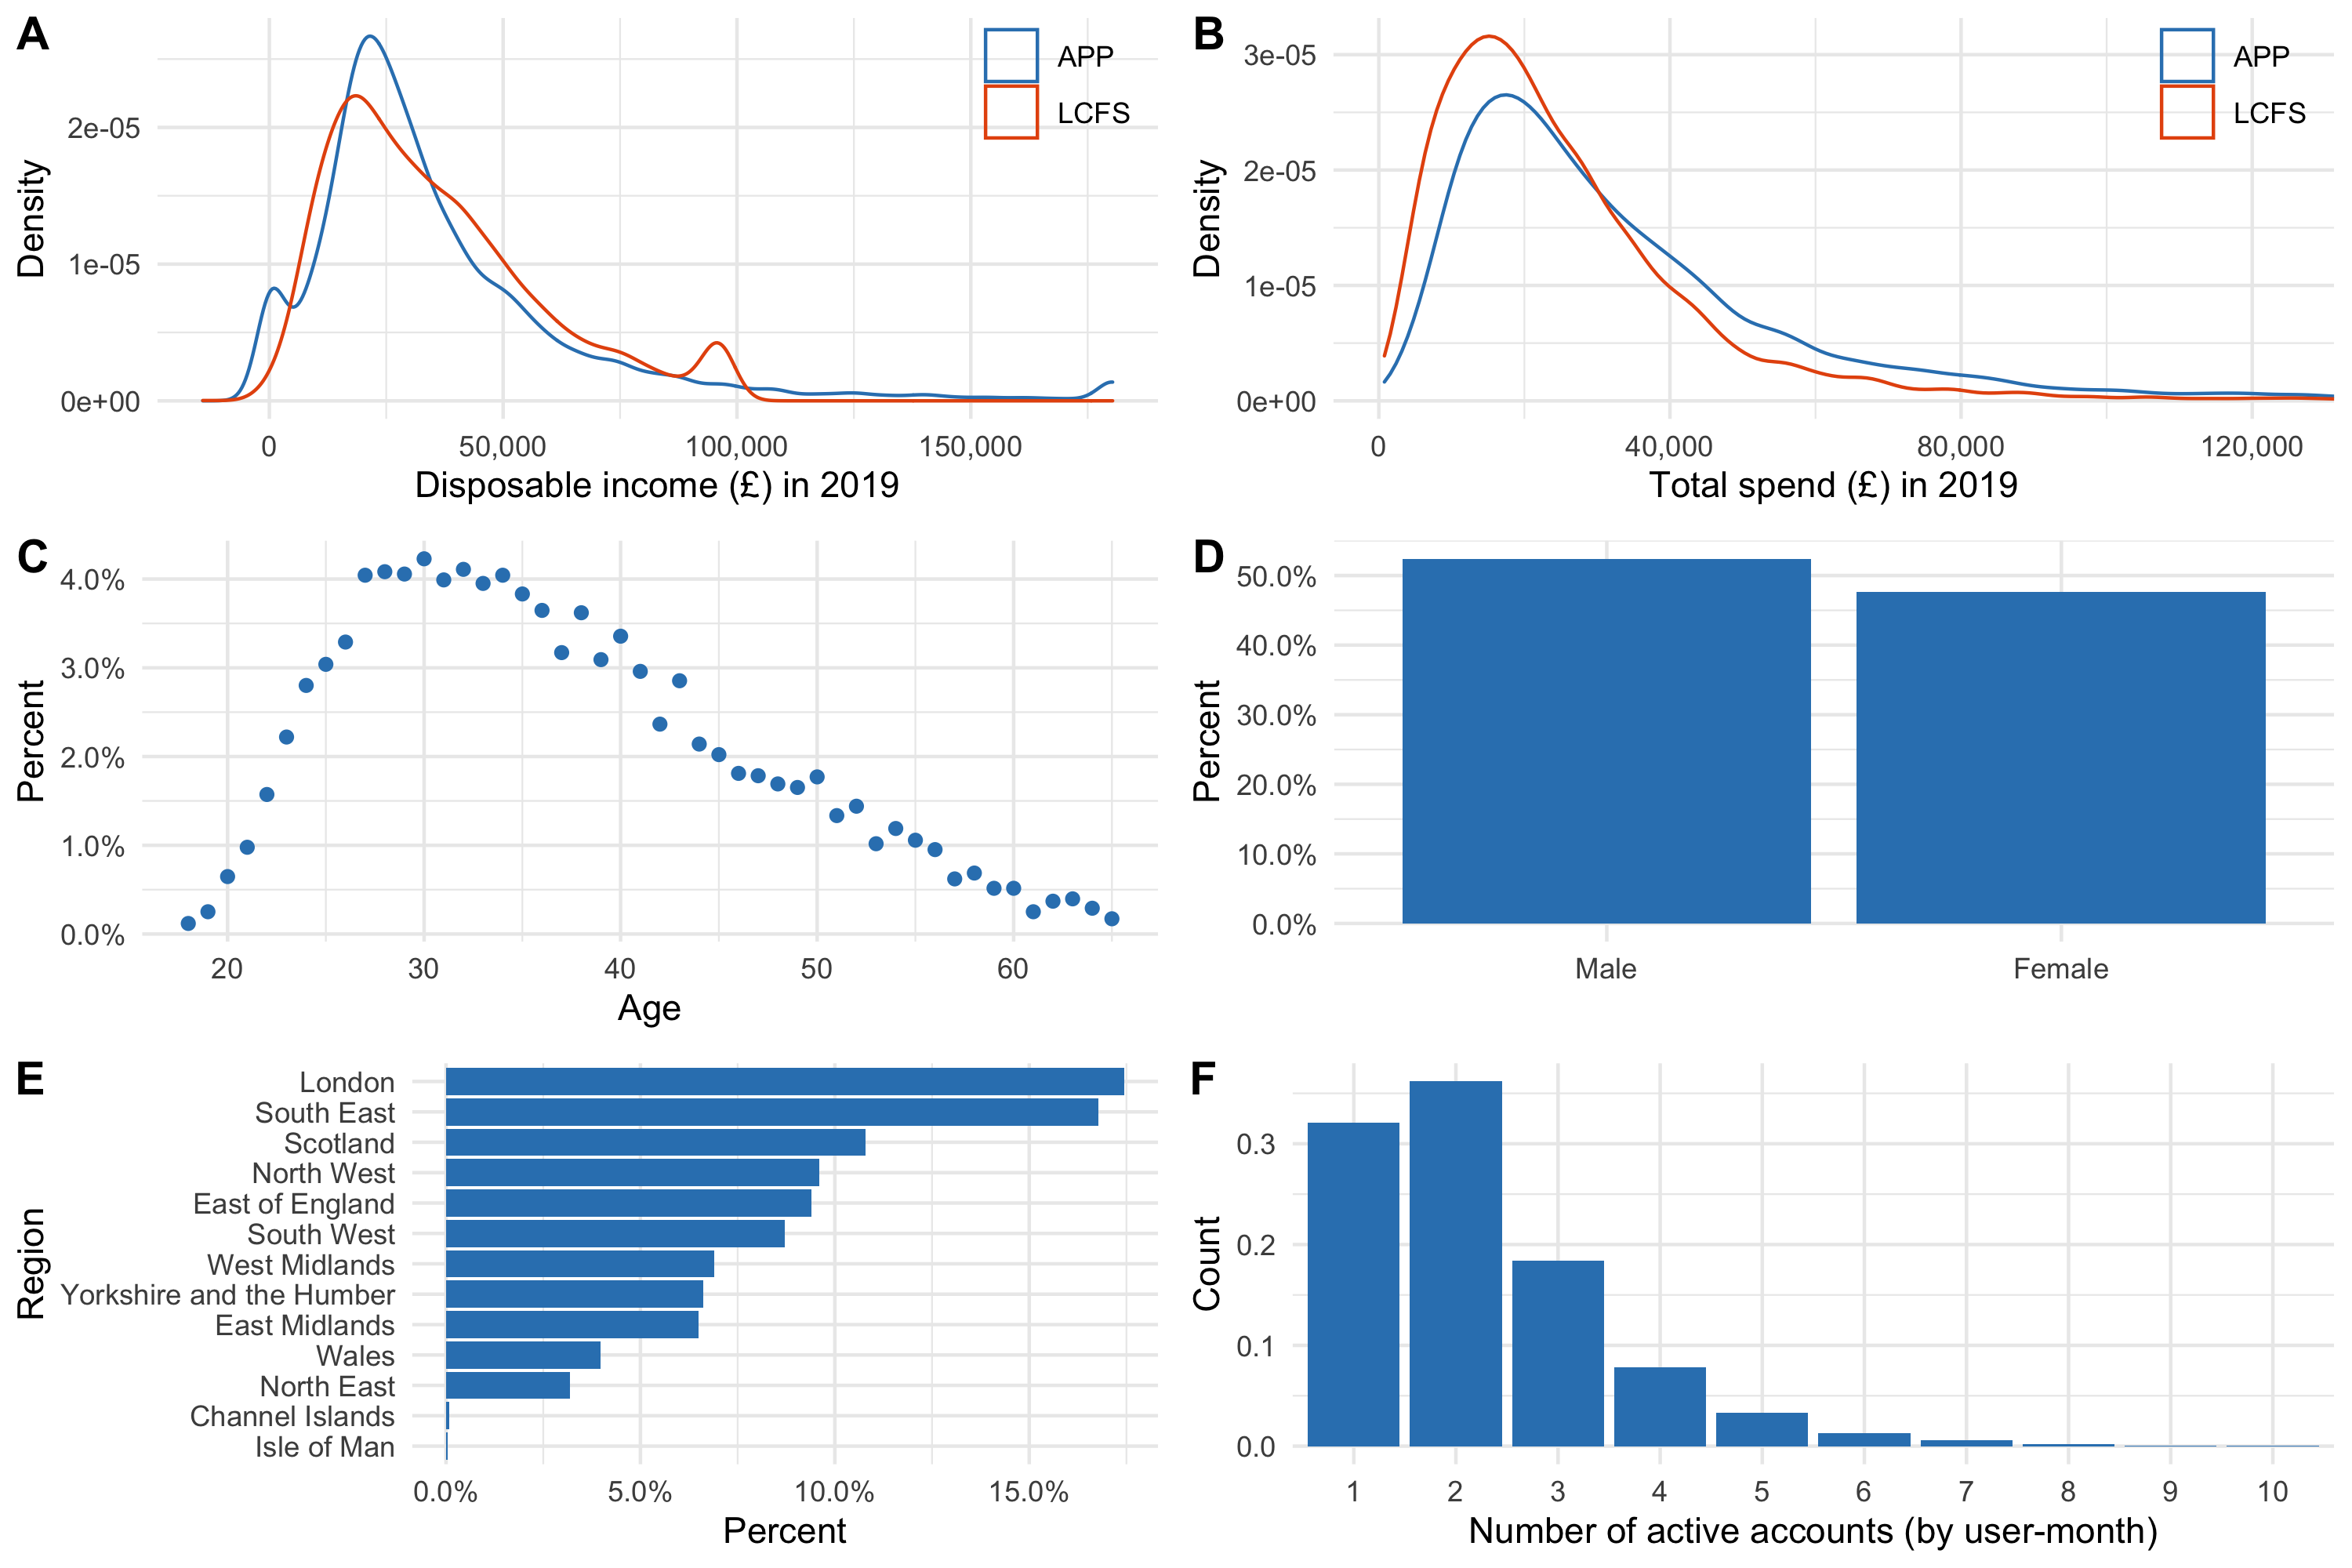
\includegraphics[width=\linewidth]{\figdir/sample_description.png}
    \label{fig:sample_description}
    \fignote{\textwidth}{Panels A and B show the distribution of disposable
        income and total spending in 2019, respectively, benchmarked against
        the 2018/19 wave of the ONS Living Cost and Food Survey (LCFS). The
        remaining panels show the data distributions of age, gender, region,
    and the number of active accounts.}%
\end{figure}

Table~\ref{tab:sumstats} provides summary statistics.


\begin{table}[htbp]
   \centering
   \tiny
   \begin{threeparttable}[b]
      \caption{\label{tab:reg_compare} Regression results}
      \begin{tabular}{lcccccc}
         \tabularnewline \midrule \midrule
         Dependent Variable: & \multicolumn{6}{c}{Net-inflows}\\
         Model:                     & (1)                   & (2)                & (3)                & (4)                & (5)               & (6)\\  
         \midrule
         \emph{Variables}\\
         App use                    & 14.330$^{**}$         & 15.303$^{***}$     & 15.303$^{***}$     & 19.381$^{***}$     & 15.963$^{**}$     & 20.207$^{***}$\\   
                                    & [2.650; 26.009]       & [3.686; 26.919]    & [3.686; 26.919]    & [7.110; 31.652]    & [1.881; 30.045]   & [7.940; 32.473]\\   
         Month income               &                       & 0.053$^{***}$      & 0.053$^{***}$      & 0.060$^{***}$      & 0.053$^{***}$     & 0.058$^{***}$\\   
                                    &                       & [0.049; 0.058]     & [0.049; 0.058]     & [0.045; 0.075]     & [0.045; 0.060]    & [0.043; 0.073]\\   
         Month spend                &                       & -0.077$^{***}$     & -0.077$^{***}$     & -0.100$^{***}$     & -0.076$^{***}$    & -0.098$^{***}$\\   
                                    &                       & [-0.081; -0.073]   & [-0.081; -0.073]   & [-0.109; -0.091]   & [-0.091; -0.061]  & [-0.107; -0.089]\\   
         Disc. spend                &                       & 138.940$^{***}$    & 138.940$^{***}$    & 169.002$^{***}$    & 132.862$^{***}$   & 156.441$^{***}$\\   
                                    &                       & [115.597; 162.282] & [115.597; 162.282] & [128.874; 209.129] & [90.975; 174.750] & [115.907; 196.976]\\   
         Female                     &                       & -14.521$^{***}$    & -14.521$^{***}$    &                    & -14.247$^{***}$   &   \\   
                                    &                       & [-24.998; -4.044]  & [-24.998; -4.044]  &                    & [-21.206; -7.289] &   \\   
         Generation $=$ GenX        &                       & 39.071$^{***}$     & 39.071$^{***}$     &                    & 39.379$^{**}$     &   \\   
                                    &                       & [19.258; 58.885]   & [19.258; 58.885]   &                    & [9.611; 69.148]   &   \\   
         Generation $=$ Millennials &                       & 71.330$^{***}$     & 71.330$^{***}$     &                    & 71.699$^{***}$    &   \\   
                                    &                       & [51.964; 90.697]   & [51.964; 90.697]   &                    & [40.338; 103.060] &   \\   
         Generation $=$ GenZ        &                       & 42.302             & 42.302             &                    & 43.095$^{*}$      &   \\   
                                    &                       & [-9.381; 93.985]   & [-9.381; 93.985]   &                    & [-7.002; 93.192]  &   \\   
         Intercept                  & -20.523$^{***}$       & -59.208$^{***}$    & -59.208$^{***}$    &                    &                   &   \\   
                                    & [-30.679; -10.368]    & [-84.179; -34.237] & [-84.179; -34.237] &                    &                   &   \\   
         \midrule
         \emph{Fixed-effects}\\
         User FE                    &                       &                    &                    & Yes                &                   & Yes\\  
         Month FE                   &                       &                    &                    &                    & Yes               & Yes\\  
         \midrule
         \emph{Fit statistics}\\
         Observations               & 184,847               & 184,847            & 184,847            & 184,847            & 184,847           & 184,847\\  
         R$^2$                      & $3.13\times 10^{-5}$  & 0.01132            & 0.01132            & 0.10137            & 0.01203           & 0.10203\\  
         Within R$^2$               &                       &                    &                    & 0.00905            & 0.01117           & 0.00885\\  
         \midrule \midrule
         \multicolumn{7}{l}{\emph{Signif. Codes: ***: 0.01, **: 0.05, *: 0.1}}\\
      \end{tabular}
   \end{threeparttable}
\end{table}




We use data from the 2018-2019 wave of the Office of National Statistics' Living Costs and Food
Survey (LCFS).\footnote{We accessed the data via the UK Data Service at the
following url:
\url{https://beta.ukdataservice.ac.uk/datacatalogue/studies/study?id=8686}.}
Data covers the period between April 2018 and March 2019.


\subsection{Estimation}%
\label{sub:estimation}

We want to estimate the effect of app use over time.  Given our data, a natural
way to do this would be to use a dynamic two-way fixed effects model that
includes user and year-month fixed effects and dummies indicating time since
app signup. The estimated coefficients on these dummies are then conventionally
interpreted as dynamic treatment effects. However, a series of recent papers
have documented that while such an approach is frequently used in applied
research, the parameter estimates from dynamic two-way fixed effects models are
not valid estimators of dynamic treatment effect in most settings. In
particular, in settings with staggered treatment assignment, where units are
first exposed to treatment at different points in time (as is the case in our
setting), dynamic two-way fixed effects are valid only if there is homogeneity
in treatment effects across treatment adoption cohorts. In most settings,
including our own, this is a very strong assumption.\footnote{Two excellent
reviews of this new literature are \citet{roth2022trending, baker2022much}.}

Because of this, I use a new estimator proposed by
\citet{callaway2021difference}, which allows for arbitrary treatment effect
heterogeneity across treatment adoption cohorts and time, and allows for the
incorporation of a parallel trends assumption conditional on covariates. In
describing the estimator, I follow the approach of
\citet{callaway2021difference} of first defining the causal parameter of
interest, and then discussing identification, estimation, and inference.

The basic building block of the framework, and the causal effect of interest,
is the group-time average treatment effect: the average treatment effect at
time $t$ for the group of individuals first treated at time $g$, defined as:

\begin{equation}
    ATT(g,t) = \mathop{\mathbb{E}}[Y_{i,t}(g) - Y_{i,t}(0)|G_i =
    g],
\end{equation}

where $Y_{i,t}(g)$ is the potential outcome in time period $t$ of an individual
$i$ in group $g$, and $Y_{i,t}(0)$ is the (counterfactual) potential outcome of that same
individual if they had remained untreated.

These effects are identified if two main assumptions hold: if there is limited
and known anticipation of treatment, and if the assumption of parallel trends
between treatment and comparison groups holds either unconditionally or
conditionally on a set of covariates.\footnote{Additional assumptions are (i)
    that the treatment is absorbing in the sense that once an individual is
    treated they will remain treated forever, (ii) that individuals in the data
    are randomly and independently drawn from a larger population, and (iii) an
    overlap condition that ensures that there is a positive number of users
    that is first exposed to the treatment at any period and that -- under the
    conditional parallel trends assumption -- propensity scores for initial
    treatment times based on covariates are bounded away from zero. The first
    assumption could be violated only if a user closes their account on the app
    and then signed up again later on, all within the roughly within the
    two-year data periods I use. This cannot be more than a tiny minority of
    users.  The second assumption holds less trivially. One way to think of a
    super population from which the users in the dataset are drawn is to think
    of knowledge about the app as partially random, and about the super
    population of all individuals who would have signed up had they learned
    about the apps existence.} Because the purpose of this section is to convey
    the core idea of the estimation approach, I keep things as simple as
    possible and discuss only the case with no anticipation effects and where
    the parallel trend assumption holds unconditionally.
    \citet{callaway2021difference} show that the same overall approach also
    works when allowing for known anticipation and conditional parallel
    trends.\footnote{Intuitively, known anticipation merely shifts the
        reference period from the period immediately before treatment to the
        period before anticipation of treatment begins. When relying on the
        conditional parallel trends assumption, the overall the group-time
        average treatment effect $ATT(g, t)$ is the average of unconditional
        group-time average treatment effects for each value of the covariate
        vector $X_i$.  As discussed in \citet{roth2022trending}, estimation is
        challenging when $X_i$ is continuous or can take on a large number of
        values, since then we will typically lack data to estimate
        unconditional group-time treatment effects for each value of $X_i$.
        There are different semi- and non-parametric approaches that can be
        used in such cases. Below, I use the doubly-robust estimator, which is
    the default in the `did` package. See \citet{callaway2021difference,
roth2022trending} for more details.}

Given these two assumptions, \citet{callaway2021difference} show that
$ATT(g,t)$ is identified by comparing the expected change of group $g$ between
periods $t$ and $g-1$ with that of a comparison group that is not yet treated
at time $t$:

\begin{equation}
    ATT(g,t) = \mathop{\mathbb{E}}[Y_{i,t} - Y_{i,g-1}|G_i = g] -
    \mathop{\mathbb{E}}[Y_{i,t} - Y_{i,g-1}|G_i = g'], \text{ for any $g'$ > t} 
\end{equation}

As this holds for all $g'$ that are not yet treated at time $t$, it also holds
for an average over all groups in the set $\mathcal{G}$ containing all groups
$g'$ for which $g' > t$,

\begin{equation}
    ATT(g,t) = \mathop{\mathbb{E}}[Y_{i,t} - Y_{i,g-1}|G_i = g] -
    \mathop{\mathbb{E}}[Y_{i,t} - Y_{i,g-1}|G_i \in \mathcal{G}].
\end{equation}

This equation encapsulates two main results: that the period just before
treatment, $g-1$, is a valid reference period, and that the group of all
individuals that have not yet been treated at time $t$ are a valid comparison
group for estimating treatment effects in time $t$.\footnote{If a group of
never-treated individuals is available, then these could also serve as a
comparison group. But because my dataset does not contain such individuals, I
do not discuss this case.} As a result of this, units who are treated in the
very first period in the dataset are dropped from the sample, since there
exists no possible control group based on which to identify their treatment
effect, and since they are not useful as a control group themselves. Similarly,
unit treated in the very last period in the data are also dropped, since there
exists no ``not-yet-treated`` group that could serve as a comparison group for
them.

$ATT(g,t)$ can then be estimated by replacing expectations with their sample
analogues,

\begin{equation}
    \widehat{ATT(g,t)} = \frac{1}{N_g}\sum_{i:G_i=g}[Y_{i,t} - Y_{i, g-1}] -
    \frac{1}{N_\mathcal{G}}\sum_{i:G_i \in \mathcal{G}}[Y_{i,t} - Y_{i, g-1}]
\end{equation}

Once these building blocks are estimated, aggregating them to event-study type treatment effects that provide the (weighted)
average treatment effect $l$ periods away from treatment adoption across
different adoption groups can be achieved by simply calculating

\begin{equation}
    ATT_l = \sum_g w_g ATT(g,g+l),
\end{equation}

where the group weights $w_g$ are the groups relative frequencies in the
treated population. When calculating these event study parameters, I use a
panel balanced in event times, with all units being observed for at least 5
treatment periods. This avoids the $ATT_l$ being influenced by different
group compositions at different periods $l$.\footnote{See Section 3.1.1 in
\citet{callaway2021difference} for a more detailed discussion.}


\subsection{Variables}%
\label{sub:variables}



\paragraph{Treatment}%
\label{par:treatment}

A user changes treatment status from untreated to treated when they start using
the app. Figure~\ref{fig:treatplot_sample_raw} shows the treatment history for
200 randomly selected users.

\begin{figure}[H]
    \centering
    \caption{Treatment assignment plot}%
    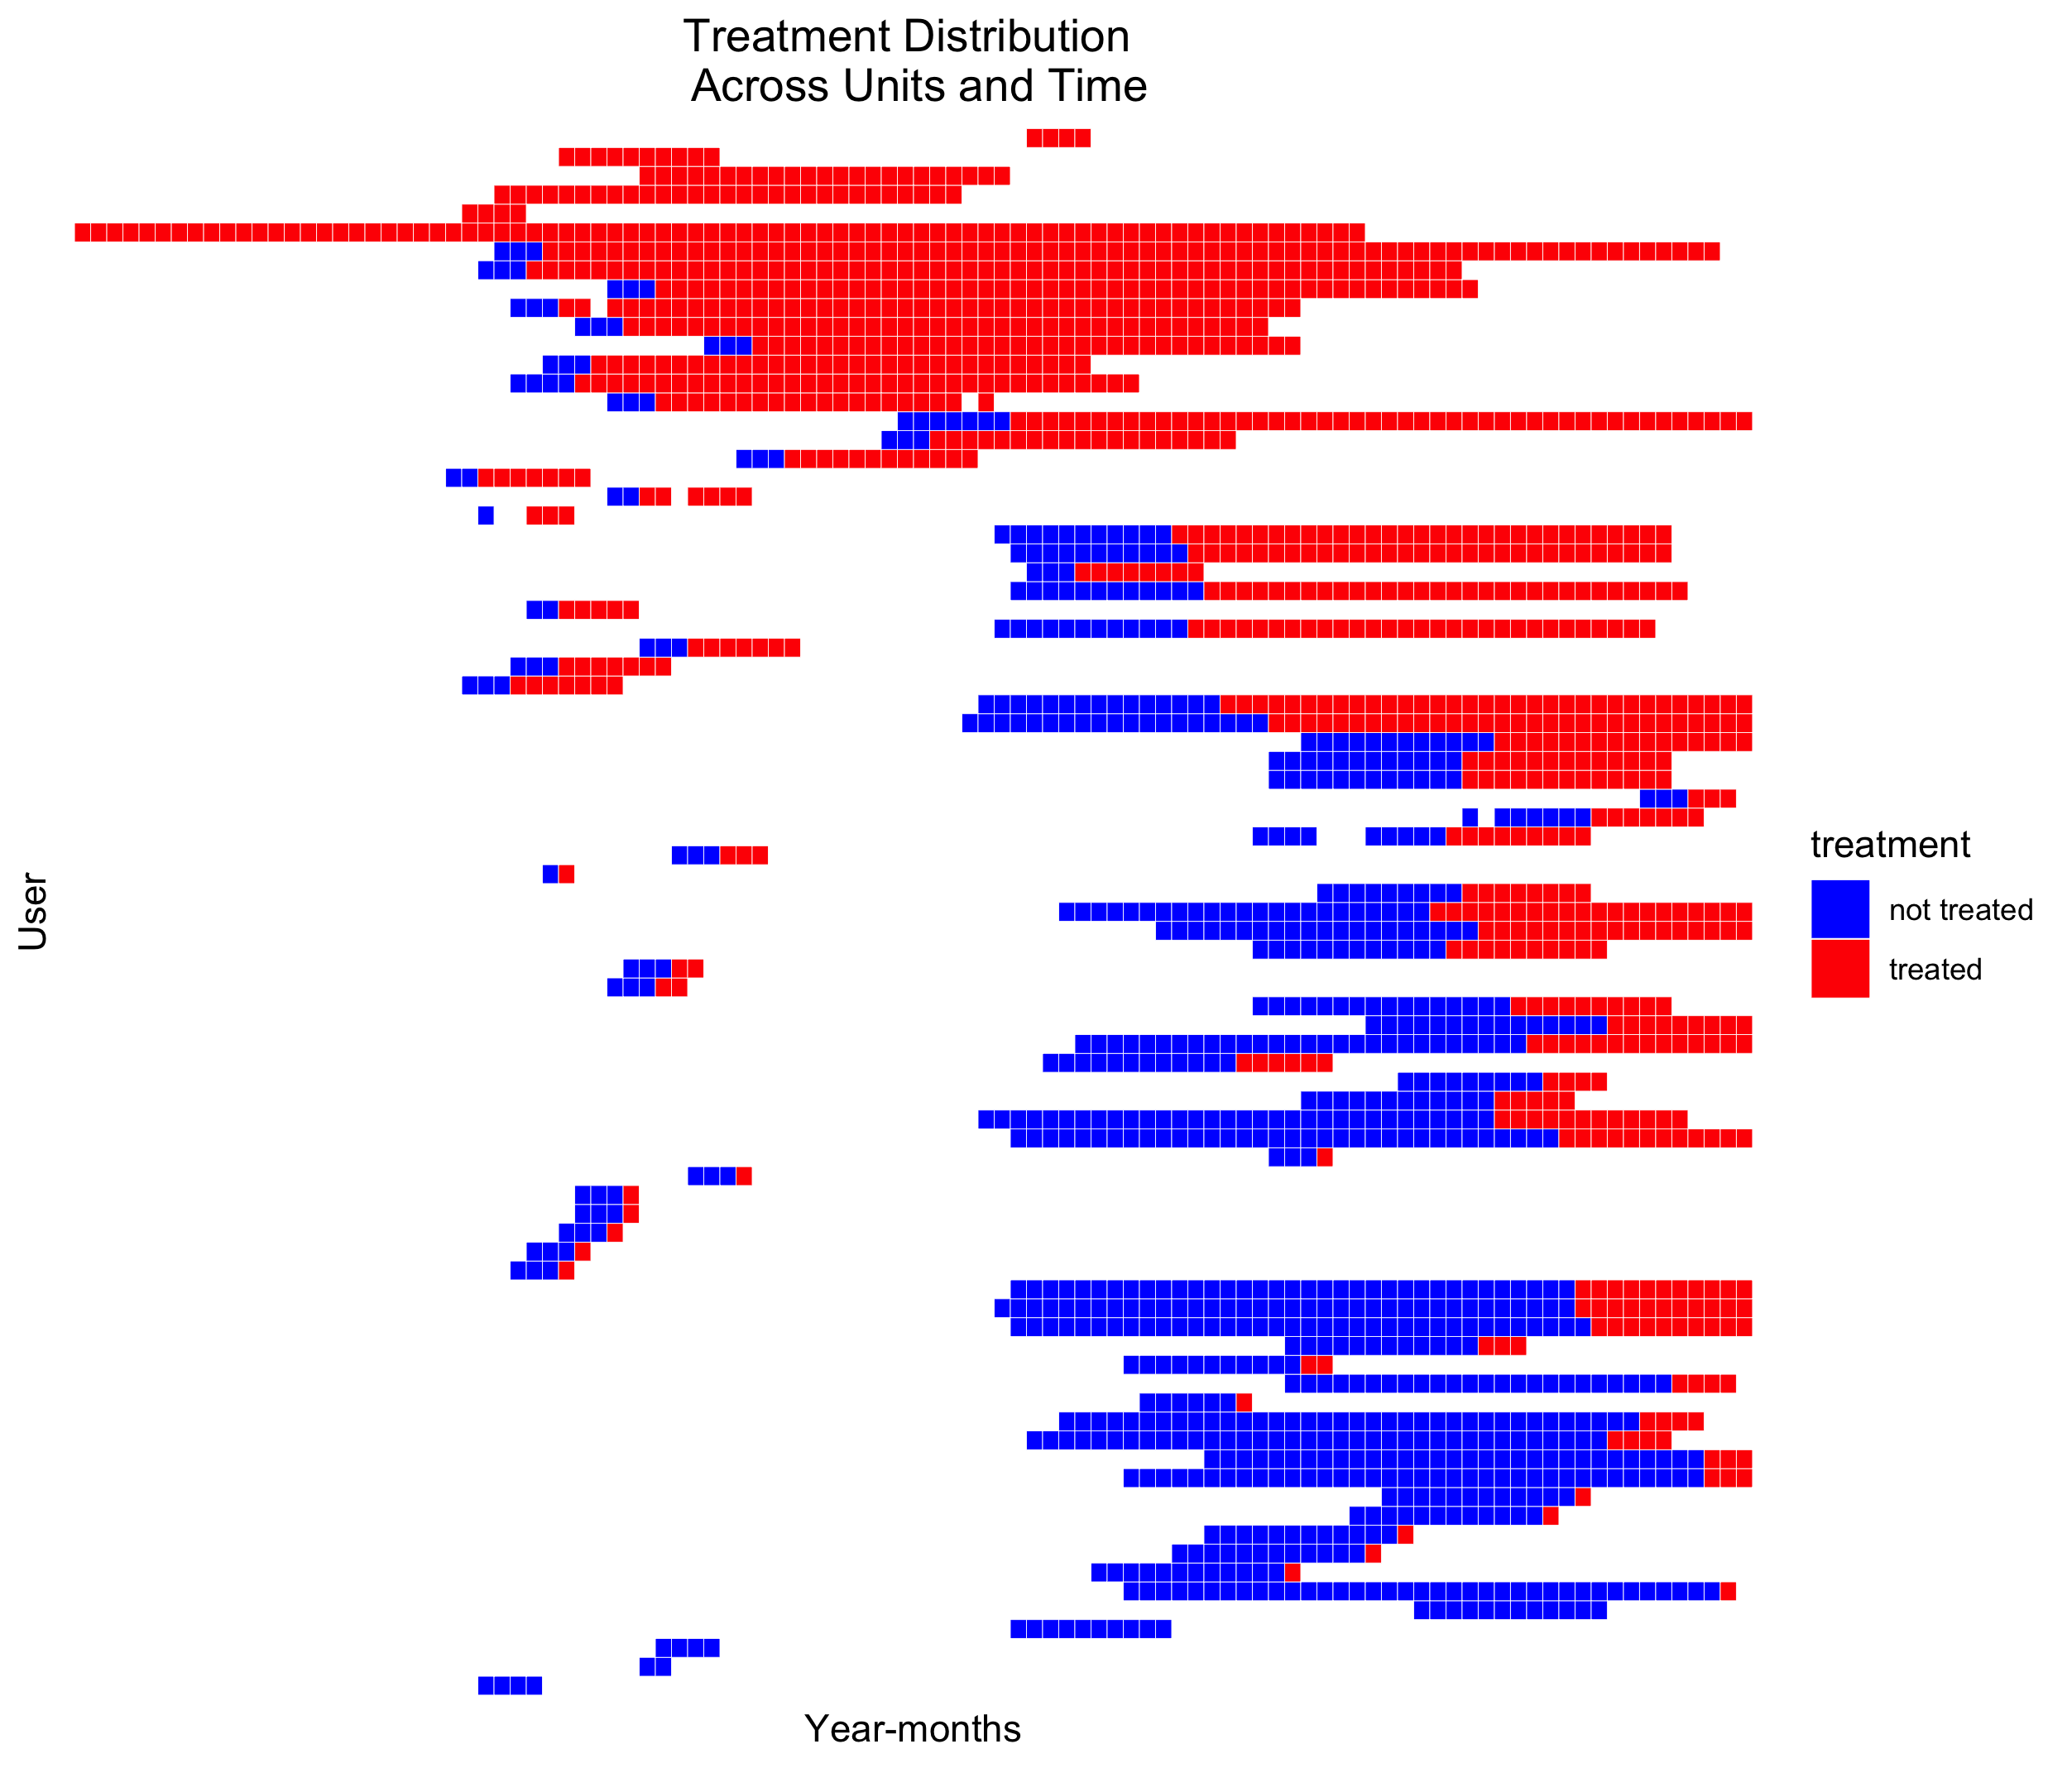
\includegraphics[width=0.8\linewidth]{\figdir/treatplot_sample_raw.png}
    \label{fig:treatplot_sample_raw}

    \fignote{\textwidth}{Each horizontal line shows the observed pre and post
        signup periods in blue and red, respectively, for one of 200 randomly
        selected users. The faint vertical white lines indicate month borders,
        whitespace indicates periods in which we do not observe the user. To
    the left of the observed period, this is because the app cannot access data
before that point when the user signs up; to the right, because they have
stopped using the app.}

\end{figure}


\paragraph{Outcomes}%
\label{par:outcomes}

Savings... see Table~\ref{tab:vars} for details.

For a more nuanced understanding of how app use affects savings we also
consider net-savings -- total savings account inflows minus outflows -- as a
proportion of monthly income to see whether a willingness to save more might be
offset by a (later) need to withdraw funds, and a dummy variable for whether a
user has any savings account inflows in a given month to see whether the app
helps users save at all. To investigate possible channels, we consider total
spend, highly discretionary spend, banking charges, the total amount of
borrowing, as well as payday borrowing, all as proportion of monthly income.



Net savings (\textit{netflows\_norm})
Inflows into minus outflows out of all of a user's savings accounts divided
by monthly income. To capture only ``user-generated'' flows, we exclude
interest and ``save the change'' transactions, as well as transactions of
less than \pounds5 in absolute
value. Monthly income and raw inflows and outflows are winsorised at the 1
percent level.
We focus on net inflows to capture effective savings.

Positive net savings dummy (\textit{has\_pos\_netflows})
Dummy equal to 1 if there were positive net savings (as defined above).
Captures extensive margin of savings (change in number of months with positive
net deposits)

Positive net savings (\textit{pos\_netflows})
Equal to net savings if there were positive net savings.
Captures intensive margin of savings (change in deposit amount in months with
positive net deposits)

\begin{figure}[H]
    \centering
    \caption{Savings patterns}%
    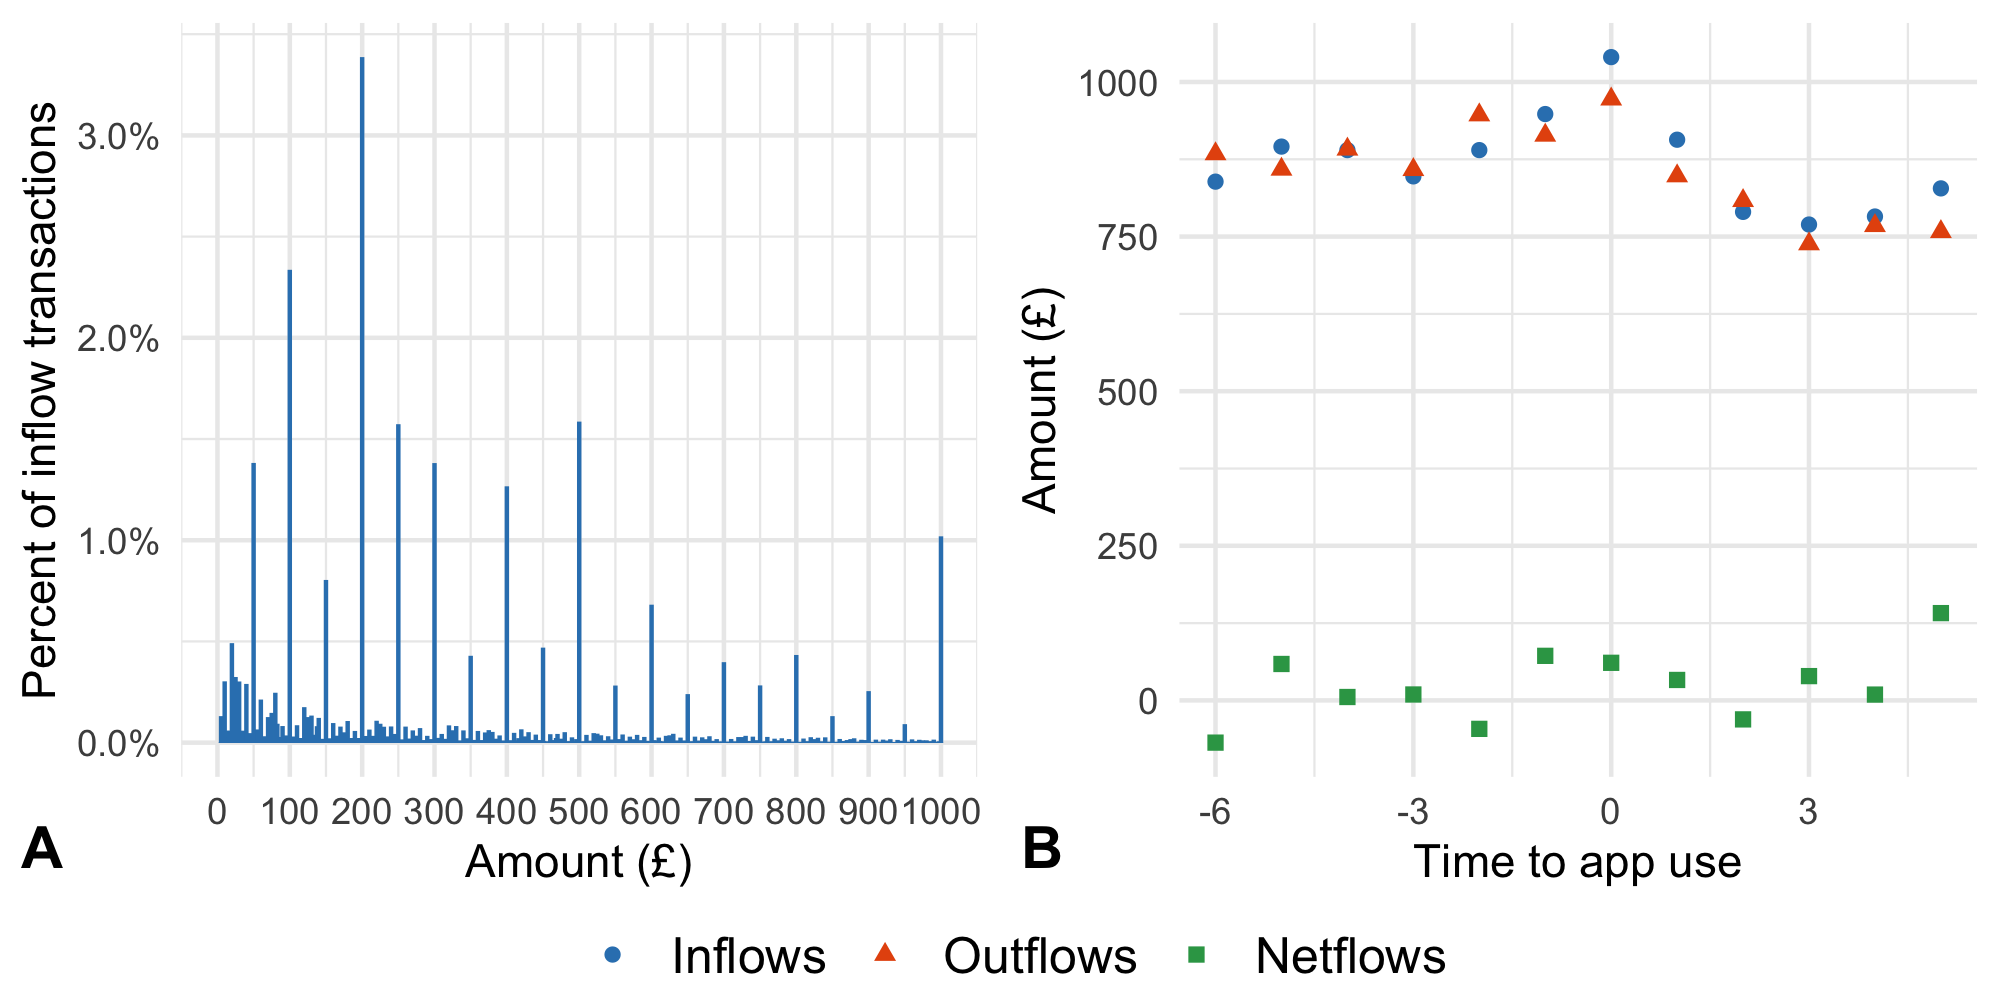
\includegraphics[width=\linewidth]{\figdir/savings_patterns.png}
    \label{fig:\figdir/savings_patterns}
    \fignote{\textwidth}{Panel A shows distribution of savings account inflow
        amounts, making clear that most transactions are the kinds of round
        amounts we would expect savings transactions to be. The data is
        truncated at \pounds1000. Panel B hows inflows, outflows, and netflows
        into savings accounts for six months before and five months after app
    use.}

\end{figure}


% \paragraph{Adjusting for multiple hypothesis tests}%
% \label{par:adjusting_for_multiple_hypothesis_tests}
% We think of our secondary outcomes as exploratory and do not make any
% adjustments for multiple hypothesis testing.\footnote{For a recent
% game-theoretically motivated discussion of when and how to correct for multiple
% hypothesis testing, see \citet{viviano2021should}.} An alternative approach,
% based on \citet{anderson2008multiple}, would be to group outcomes into
% ``savings'', ``spending'', ``borrowing'', and ``fees'', and consider them as
% different dimensions of a latent variable of interest which we might call
% ``financial management skills''. We do not do that for two reasons: first and
% foremost, because we think it is natural to think of the amount saved as the
% ultimate outcome and of other outcomes as providing a more nuanced
% understanding of savings behaviour or as suggesting possible channels through
% which app use affects savings. Thinking of savings as the main goal is also
% reflected in Money Dashboard's main promise, which is to help users spend less
% and save more, as shown in Figure~\ref{fig:mdb_website}. Second, as pointed out
% in \citet{carlin2017fintech}, incurring overdraft fees is not an unambiguous
% sign of a financial mistake, as the opportunity to go into overdraft confers a
% benefit to the consumer.\footnote{For further discussions on fees, see
% \citet{jorring2020financial, stango2009consumers}.}


\paragraph{Covariates}%
\label{par:covariates}

We control for baseline behaviour, events, and personal characteristics that,
to various degrees, capture a person's need, capacity, motivation, and
awareness to save. Table~\ref{tab:vars} lists all covariates used
together with their definition and the rationale for including them. For all
variables, we include contemporaneous values as well as lags for up to 6
periods. In addition, we control for the previous six months of savings to
capture time-invariant unobserved drivers of savings behaviour (in
specifications without fixed effects) as well as a possible signal for a higher
or lower need for future savings.

Following \citet{vanderweele2019principles} we include covariates that affect
either outcomes or the propensity for treatment or both, exclude from this
set of variables those that are instruments (affect the outcome only through their effect on
treatment propensity) and add to it proxies for unobserved variables that are a
common cause of both outcomes and treatment propensity.\footnote{
\citet{vanderweele2019principles} calls this the ``modified disjunctive cause
criterion'' for covariate selection, as it includes the set of variables that are causally
related to either outcomes, or treatment propensity, or both, but modified to
account for potential bias by excluding instruments and including proxies of
unobserved causes of both outcomes and treatment.}

The table below describes the construction and rationale for including of all
variables used. The code used to construct the variables is available on
\href{https://github.com/fabiangunzinger/mdb_eval/blob/d094f8cd364f64bbe3d4e644abbff726af86de2f/src/data/aggregators.py}{GitHub}.

\begin{table}[htpb]
    \centering\scriptsize
    \caption{Covariates}
    \label{tab:vars}
    \begin{tabularx}{\textwidth}{>{\raggedright\arraybackslash}X
        >{\raggedright\arraybackslash}X>{\raggedright\arraybackslash}X}
    \hline\hline
    Variable (name in dataset) & Definition  & Rationale \\
    \hline\\
    \multicolumn{3}{c}{\textbf{Primary outcome}}\\\\

    \multicolumn{3}{c}{\textbf{Covariates}}\\\\

    New loan dummy (\textit{new\_loan})&
    Dummy variable equal to 1 if user takes out a new loan. Calculated positive inflows
    of funds tagged as ``loan''.&
    Might increase (additional funds) or decrease (need to repay) propensity to
    save in month of takeout and lower propensity to save in the future due to
    need to repay.\\

    Unemployment benefits dummy (\textit{unemp\_benefits})&
    Dummy variable equal to 1 if user has inflow of funds tagged as ``job
    seeker benefits''.&
    Might lower a user's ability to save but increase their need for a money
    management app.\\

    Monthly income (\textit{month\_income})&
    Average monthly income in a calendar year, calculated as the sum of all
    credits tagged income payments in said year divided by 12.&
    Income may alter the need and ability to save and correlate with cognitive
    characteristics that alter a person's propensity to use a money management
    app.\\

    \hline\hline
    \end{tabularx}
\end{table}




\subsection{Code access}%
\label{sub:code_access}

We provide links to code that creates key elements of the paper such as
variable definitions and sample selection directly in the relevant places in
the paper so they can be accessed conveniently. The links are indicated with
the GitHub logo, \faGithub. The hope is that this helps the
curious reader clarify questions about subtleties they might have while reading
the paper. The complete projects GitHub repo is at
\href{https://github.com/fabiangunzinger/mdb\_eval}{https://github.com/fabiangunzinger/mdb\_eval}.


